% vim:ft=tex:
%
\RequirePackage[l2tabu, orthodox]{nag}
\documentclass[runningheads]{llncs}
\pagestyle{headings}


%%%%%%%%%%%%%%%%%%%%%%%%%%%%%%%%%%%%%%%
% FONTS
%%%%%%%%%%%%%%%%%%%%%%%%%%%%%%%%%%%%%%%

\usepackage{lmodern}        % Improved version of the original Computer Modern font
\usepackage{courier}
% \usepackage{times}

\usepackage[T1]{fontenc}    % Determines font encoding of the output. Font packages have to be included before this line.
\usepackage[utf8]{inputenc} % Determines encoding of the input. All input files have to use UTF8 encoding.
\usepackage[english]{babel}


%%%%%%%%%%%%%%%%%%%%%%%%%%%%%%%%%%%%%%%
% PACKAGES
%%%%%%%%%%%%%%%%%%%%%%%%%%%%%%%%%%%%%%%

\usepackage[pages=some]{background}
\usepackage{amsmath}
\usepackage{amssymb}
% \usepackage{thmtools}
% \usepackage{mathtools}
% \usepackage{prftree}
% \usepackage{cancel}
% \usepackage{keycommand}
\usepackage{listings}
\usepackage{paralist,proof}

% \usepackage{lstautogobble}
\usepackage{microtype}  % Small-scale typographic enhancements.
\usepackage[shortlabels]{enumitem}
\usepackage[hidelinks]{hyperref}  % optional argument [hidelinks] hides colored boxes around clickable areas
%\usepackage{prftree}
\usepackage{mathtools}
\usepackage{booktabs}   % Improves the typesettings of tables.
\usepackage{tabularx}
\usepackage{multirow}   % Allows table elements to span several rows.
\usepackage{pdfpages}  % to include pages from existing pdf files with \includepdf[pages={1,2}]{./path/to/file.pdf}
\usepackage{xcolor}
\usepackage{todonotes}  % Add optional argument [disable] to hide TODOs, or [obeyFinal] to hide only in final mode
\usepackage{mdframed}

\usepackage{tikz}
\usetikzlibrary{arrows, arrows.meta, backgrounds, calc, decorations.markings, positioning, shapes.geometric}


%%%%%%%%%%%%%%%%%%%%%%%%%%%%%%%%%%%%%%%
% SETTINGS
%%%%%%%%%%%%%%%%%%%%%%%%%%%%%%%%%%%%%%%

% \setlist{nolistsep}  % less vertical spacing for itemize/enumerate environments


%%%%%%%%%%%%%%%%%%%%%%%%%%%%%%%%%%%%%%%
% MACROS
%%%%%%%%%%%%%%%%%%%%%%%%%%%%%%%%%%%%%%%

\makeatletter
% \def\UrlFont{\rmfamily}
% \def\orcidID#1{\smash{\href{http://orcid.org/#1}{\protect\raisebox{-1.25pt}{\protect\includegraphics{orcid_color.eps}}}}}
% The \smash breaks the hyperlink... the clickable area becomes tiny.
\def\orcidID#1{{\href{http://orcid.org/#1}{\protect\raisebox{-1.25pt}{\protect
\includegraphics{ORCID_Color.eps}}}}}
\makeatother

\newcommand{\todoi}[1]{\todo[inline,caption={}]{#1}}    % caption={} allows itemize etc. inside todoi, see https://tex.stackexchange.com/a/54068

% This is the provability analogue to \models (note that \vdash is smaller)
\DeclareRobustCommand\proves{\mathrel{|}\joinrel\mkern-.5mu\mathrel{-}}

\newcommand{\limpl}{\rightarrow}    % logical implication
\newcommand{\Limpl}{\Rightarrow}    % logical implication (variant)
\newcommand{\liff}{\leftrightarrow} % logical equivalence
\newcommand{\Liff}{\Leftrightarrow} % logical equivalence (variant)

\newcommand{\Land}{\bigwedge}
\newcommand{\Lor}{\bigvee}

\newcommand{\union}{\cup}
\newcommand{\Union}{\bigcup}
\newcommand{\intersect}{\cap}
\newcommand{\Intersect}{\bigcap}

\newcommand{\eql}{\simeq}
\newcommand{\neql}{\not\eql}

% \newcommand{\nat}{\mathbb{N}}
% \newcommand{\int}{\mathbb{Z}}

\newcommand{\naf}{{\sim}}           % negation as failure, default negation
\newcommand{\caF}{\mathcal{F}}
\newcommand{\caM}{\mathcal{M}}
\newcommand{\caT}{\mathcal{T}}

\newcommand{\vampire}{\textsc{Vampire}}


%%%%%%%%%%%%%%%%%%%%%%%%%%%%%%%%%%%%%%%
% METADATA
%%%%%%%%%%%%%%%%%%%%%%%%%%%%%%%%%%%%%%%

\title{Automated Reasoning in Generating Exam Sheets for Automated Deduction}
\titlerunning{Automated Reasoning in Generating Exam Sheets}
\author{Petra Hozzov\'a\and
Laura Kov\'acs \and
Jakob Rath}
\authorrunning{\hspace*{-11.2em}Petra Hozzov\'a\and
Laura Kov\'acs \and
Jakob Rath}

\institute{
    TU Wien, Austria
    % \and
    % Princeton University, Princeton NJ 08544, USA \and
    % Springer Heidelberg, Tiergartenstr. 17, 69121 Heidelberg, Germany
    % \email{lncs@springer.com}\\
    % \url{http://www.springer.com/gp/computer-science/lncs} \and
    % ABC Institute, Rupert-Karls-University Heidelberg, Heidelberg, Germany\\
    % \email{\{abc,lncs\}@uni-heidelberg.de}
}

% Set PDF document properties
\hypersetup{
    pdfpagemode     = UseNone,                  % Don't show bookmarks when opening the pdf file, see also https://latex.org/forum/viewtopic.php?p=70568#p70568
    pdfpagelayout   = OneColumn,                % How the document is shown in PDF viewers (optional). Values: SinglePage, OneColumn, TwoColumnLeft, TwoColumnRight, TwoPageLeft, TwoPageRight
    % pdfauthor       = {\authorname},          % The author's name in the document properties (optional).
    % pdftitle        = {\thesistitle},         % The document's title in the document properties (optional).
    % pdfsubject      = {subject},              % The document's subject in the document properties (optional).
    % pdfkeywords     = {keyword, another keyword}, % The document's keywords in the document properties (optional).
    colorlinks,
    % linkbordercolor = {Melon},                % The color of the borders of boxes around crosslinks (optional).
    linkcolor={blue},
    citecolor={blue},
    urlcolor={blue},
}

\lstset{%
    basicstyle=\ttfamily,%
    % keywordstyle=\bfseries\color{blue},%
    columns=flexible,%
    % numberstyle=\tiny,%
    % numbersep=5pt,%
    % numbers=left,%
}


%%%%%%%%%%%%%%%%%%%%%%%%%%%%%%%%%%%%%%%
\backgroundsetup{
scale=1,
color=black,
opacity=1,
angle=0,
placement=bottom,
vshift=-1cm,
contents={%
  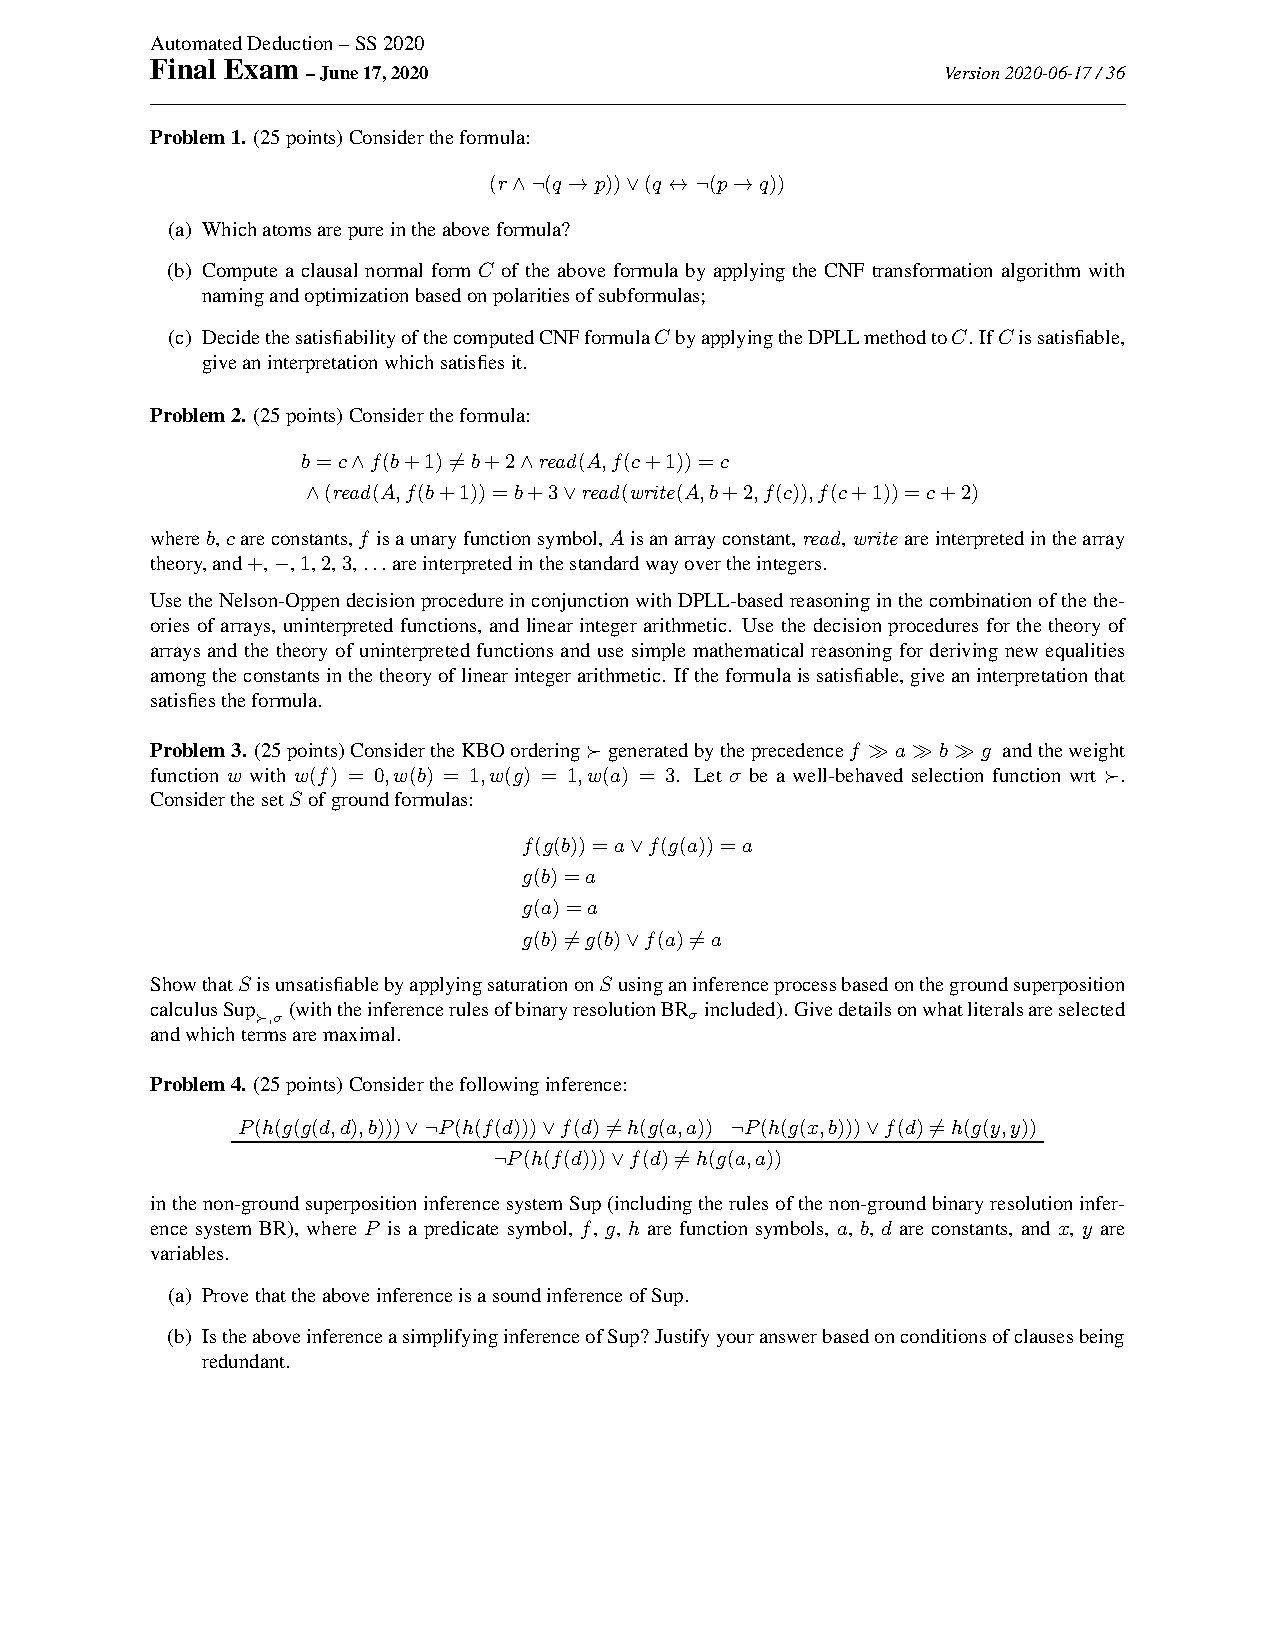
\includegraphics[page=1,width=1.5\textwidth]{./exam-36.pdf}
  }%
}

\begin{document}
\maketitle





\begin{abstract}
Amid the COVID-19 pandemic, distance teaching became default in higher education,
urging teachers and researchers to revise course materials into an
accessible online content for a diverse audience. Probably one of the hardest challenges
came with online assessments of course performance, for example by
organizing online written exams.
In this short paper we describe the online
setting  we organized for our master's level course ``Automated
Deduction'' in logic and computation at TU Wien.
The algorithmic and rigorous reasoning developed within our
course called for individual exam sheets focused on problem solving and deductive
proofs; as such exam sheets using test grids were not a viable solution
for written exams within our course.
We believe the toolchain of automated reasoning tools we have developed for
holding online written exams could be beneficial not only for other
distance learning platforms, but also to researchers in automated
reasoning, by providing our community with a large set of randomly generated benchmarks in SAT/SMT solving and first-order theorem proving.
\end{abstract}





\section{Motivation}

Amid the COVID-19 pandemic, higher education has moved to distance
teaching. While online lecturing was relatively fast to implement via
webinars, recordings,  streaming and online communication channels,
coming up with best practices to assess course performance was far
from trivial. Even with very sophisticated technical infrastructure
(use of which, on the other hand, would be unethical to require from course
participants), avoiding collusion in the virtual
environment is very hard to achieve, if possible at all.
%In addition, course assessment is very diverse and depends on the
%available resources the  institutions have to implement individual oral
%exams or large-scale written exams.
While work on
online feedback generation has already been initiated, see
e.g.~\cite{Zuleger18,Wang18}, 
not much work on online examinations has so far emerged. 

In this paper we survey our teaching-related project work in organizing online
written exams, where the exam solutions require rigorous
logical reasoning and proofs rather than using mechanized test grids.
In particular, we are faced with the challenge of organizing online
written exams for our master's level course ``Automated
Deduction'' in logic and computation at TU
Wien\footnote{\url{https://tiss.tuwien.ac.at/course/courseDetails.xhtml?dswid=2002\&dsrid=601\&courseNr=184774\&semester=2020S}}.
This course introduces algorithmic techniques and fundamental results
in automated reasoning, by focusing on specialised algorithms for
reasoning in various fragments of first-order logics, such as
propositional logic, combinations of ground theories, and full
first-order logic with equality.
As such, topics of the course cover theoretical and practical
aspects of SAT/SMT solving~\cite{DPLL,Tinelli02,DPLLT} and first-order theorem proving using
superposition reasoning~\cite{Rubio01,Vampire13}.

We claim by no means that the framework we developed for online
examination is optimal.
Given the time constraints of examination periods, we aimed for an
online exam setting that (i) reduces collusion among students and  (ii)
requires the same workload on each participant.
The algorithmic reasoning developed within our
course called for exam sheets focused on problem solving and deductive
proofs; hence, exam sheets using test grids were not a viable solution
for written exams within our course.
We have therefore used and adapted the automated reasoning approaches introduced in our
course to automate the generation of individual exam sheets for
students enrolled in our course, by making sure that the exam tasks
remain essentially the same in each generated exam sheet. As such, we have randomly generated
individual exam problems on 
\begin{itemize}
\item
    SAT solving, by imposing (mostly) syntactical constraints on
    randomly generated SAT formulas (Section~\ref{sec:sat});
    
\item Satisfiability modulo theory (SMT) reasoning, by exploiting reasoning in a combination of theories
  and varying patterns of SMT problem templates
  (Section~\ref{sec:smt});
  
\item First-order theorem proving, by adjusting simplification
  orderings in superposition reasoning and using redundancy elimination
  in first-order proving, both in the ground/quantifier-free 
  and non-ground/quantified setting (Section~\ref{sec:fo}
  and Section~\ref{sec:qf}). 
\end{itemize}

For each of the SMT and first-order problems we generated, we used respective
SMT and first-order solvers to perform an additional sanity check
(Section~\ref{sec:implementation}).
Our toolchain and the generated benchmarks/exams are available at

\begin{center}
  \url{https://github.com/JakobR/exagen}
\end{center}

We believe our framework is beneficial not only for other
distance learning platforms, but also to researchers in automated
reasoning as we provide our scientific community
a large set of randomly generated benchmarks in SAT/SMT solving and first-order theorem proving.
While our teaching-related project delivery is specific to formal aspects of automated
reasoning, we note that our work can be extended with further
constraints to scale it to other courses in formal methods. 

This paper is structured as follows. In Sections~\ref{sec:satfo}-~\ref{sec:smtqf}
we discuss the high-level approach to generating the exam
problems. Section~\ref{sec:implementation} surveys the main implementation principles supporting our
solution.
Finally, in Section~\ref{sec:comparison} we compare
the teaching outcomes of our online written exam with those coming
from previou in-class examinations. \todo{complete the summary of comparison}
%\todo{PH: Do we want to keep the section with teaching outcomes?
%JR: I would tend towards keeping it (if we can fill the remaining
%numbers for the TODOs). LK: yes, we should keep this; good for project
%survery :)}




%\section{todo}
%
%Challenge:
%problem instances should be different but of similar difficulty to make sure the exam is fair to students.



\section{Random Problem Generation}\label{sec:satfo}

We first describe our solution for generating automated reasoning
benchmarks in a fully automated and random manner. We used this
setting for generating exam problems on SAT solving and first-order
theorem proving, by 
% we discuss the two remaining problems of our exam sheet.
%For these problems, we generate instances randomly,
filtering out exam problem instances that are either too
hard or too easy. Throughout this paper, we assume basic familiarity with standard first-order
logic and refer to the literature~\cite{SAT09,Vampire13} for further details.


\subsection{Boolean Satisfiability (SAT)}\label{sec:sat}

% We describe our random generation of exam problems on SAT solving by
% first
% showing  one generated SAT exam problem, as
% below.
In our exam problem on SAT solving, students were asked to
(a) determine which atoms are of pure polarity in the formula,
(b) compute a polarity-optimized clausal normal form~\cite{Tseytin70},
and (c) decide satisfiability of the computed CNF formula by applying the DPLL algorithm.
% Thus, our task for this problem was to generate suitable propositional formulas.

Randomly generating propositional formulas in a naive setting would lead
to a huge variety of formulas,
spanning both formulas for which the above questions on SAT solving
are trivial to answer (e.g. clauses as propositional tautologies)
and others requiring much more effort
(e.g. arbitrary formulas using only $\leftrightarrow$).
More work was thus needed to
ensure comparable workload for solving exam sheets.
%This is obviously undesirable in an exam setting,
%where the tasks should ultimately be challenging, but still solvable by hand.
Furthermore,
the variation in difficulty between different exams should be kept as small as possible,
to make the setting as fair to the examinees as possible.

To this end,
we identified several  syntactical characteristics that the exam problems on SAT solving should exhibit,
and filtered the generated formulas by these, as summarized  partially
below. \smallskip
%
% The criteria are the following:
% Size: 7 connectives
% [ numAtoms fm == 3
% , -- there is at least one atom with pure polarity
%   hasAtomPolarity Neg fm || hasAtomPolarity Pos fm
% , not (anySubformula isNestedNot fm)
% , -- at least one but at most two equivalences
%   let n = countSubformulas isIff fm
%   in 1 <= n && n <= 2
% , anySubformula isImp fm
% , anySubformula isNot fm
% , anySubformula isAnd fm || anySubformula isOr fm
% , not (anySubformula isTrivialBinaryConnective fm)
% , hasVarietyInDefinitionalNF fm
% , length (models fm) <= 6
% , nestedLatexParens fm < 3
% ]

%\begin{compactenum}
\noindent(1) %    \item
        The SAT formula contains exactly seven logical connectives 
        and exactly three different propositional variables. \smallskip
        % (but each of these may appear multiple times).
    % \item
    %     The formula contains exactly seven connectives.
    % \item
    %     The formula contains exactly three different atomic propositions
    %     (but each of these may appear multiple times).

\noindent(2)        
%    \item\label{item:polarity}
        There is at least one atom that appears with a pure polarity.\smallskip
        % (i.e., either only in positive position or only in negative
        % position).
        
\noindent(3) %   \item
        The connectives ``$\leftrightarrow$'', ``$\rightarrow$'', and ``$\lnot$'' appear at least once,
        with ``$\leftrightarrow$'' appearing at most twice.
        At least one of ``$\land$'' and ``$\lor$'' appears. \smallskip
    % \item
    %     The connective ``$\leftrightarrow$'' appears at least once but at most twice.
    % \item
    %     The connectives ``$\rightarrow$'' and ``$\lnot$'' appear at least once.
    % \item
    %     At least one of the connectives ``$\land$'' or ``$\lor$''
    %     appears in the formula.
        
%LK commented out these 2
    %   \item
%        There is no subformula for the form $\lnot \lnot \varphi$ for any formula $\varphi$.
%    \item
 %       There are no trivial binary subformulas such as $p \land
 %       \lnot p$ or $p \lor p$.
 %       LK end
        
    % \item
    %     If a binary connective has a literal as argument,
    %     the other argument cannot also be a literal containing the same atomic proposition.
    %     % No binary connective has two literals that contain the same atomic proposition.
    %     % There is no binary connective that
    %     For example, this excludes subformulas such as $p \land \lnot p$ and $p \lor p$,
    %     but not $p \rightarrow q$.

\noindent(4)
        The polarity-optimized clausal normal form results in a set of definitions,
        each of which is of the form
        $n \circ \varphi$ with $\circ \in \{ \rightarrow, \leftarrow, \leftrightarrow \}$,
        a fresh propositional variable~$n$, and a formula~$\varphi$.
        We restrict the SAT formula such that at least two of the choices for
        $\circ$ appear in the clausal normal form (CNF). \smallskip

\noindent(5)
\todo{leave out this point if we need space? (if yes, also change sentence in appendix/impl about implementation efficiency where we refer to this)}
        The SAT formula has at most $6$ models.
        Since there are $2^3 = 8$ different interpretations,
        this means the formula is not valid.\smallskip

        % Note that there are $2^3 = 8$ different interpretations of our formula,
        % so this means the formula is not valid.
        % \todo{the value of this is restriction isn't clear to me anymore… I wanted to control DPLL branching somewhat but now I don't think it does anything for that.}

% \noindent(6)
%         To avoid accidental difficulty introduced by visual complexity,
%         the \LaTeX{} rendering of the formula should have a parenthesis nesting level of at most two.\smallskip
%\end{compactenum}

While the combination of the above conditions might seem very restrictive,
we note that 
%Thus, we enumerated the sample space to see how much variety is possible:
%as it turns out,
there are $20\,390\,076$ different SAT formulas satisfying the above
criteria. Further, 
if we do not want to distinguish formulas that differ only by a permutation of atoms,
$3\,398\,346$ formulas remain. Thus, we are able to generate a large
number of unique SAT formulas to be used in online examinations and
beyond.





\subsection{Non-Ground Superposition with Redundancy}\label{sec:fo}

Moving beyond boolean satisfiability, we developed a random problem
generator for first-order formulas with equality, in the setting of
superposition-based first-order theorem proving with redundancy elimination~\cite{Rubio01,Vampire13}.
In this problem, a concrete inference\footnote{i.e., an instance of an inference rule as opposed to the rule itself}
was given to the students, and their task was to
(a) prove that the inference is sound
and (b) that the inference is a simplification inference.
% We illustrate the first-order reasoning task of our
% exam in our randomly generated Example~\ref{ex:fo}.

% For generating first-order reasoning problems similar to
% Example~\ref{ex:fo}, we randomized problem generation in the setting
% of simplification inferences within saturation-based theorem
% proving.
We recall that a simplification inference is an inference
that removes clauses from the proof search space, whereas a generating
inferences add new clauses to the search space~\cite{Vampire13}. In our work, we
considered the simplification inference of 
\emph{subsumption resolution} 
\begin{equation}\label{eq:sr}
    \infer[]{
      D
      }{
      A\vee C
      &
      {\neg B \vee D}
    }
    \qquad \text{or}\qquad
  %
    \infer[]{
      D
      }{
      \neg A\vee C
      &
      {B \vee D}
    }
      \end{equation}
      where $A,B$ are atoms and $C,D$ are clauses
      such that for some substitution (or mgu) $\theta$ we have $A\theta\vee
C\theta\subseteq B\vee D$, and hence the second premise $\neg B \vee
D$ (or $B \vee
D$) of~\eqref{eq:sr} is redundant and can  be deleted from the search
space after applying~\eqref{eq:sr} within proof search.
%
We randomly generated first-order instances of the inference rule~\eqref{eq:sr}, as
discussed next. Our setting could however be easily extended to other
simplification inferences such as subsumption demodulation~\cite{Rath20},
and even generating inferences.

\noindent (1) To randomly generate first-order terms and literals,
we fix  a first-order signature consisting of % three sets specifying the allowed
predicate and function symbols and specify a set of logical
variables. 
%variables.  % (with arity),
%function symbols, % (with arity),
%and variables.
We control the shape of the generated terms
by giving bounds on the \emph{depth} of the term,
that is the maximal nesting level of function calls
(e.g., a constant symbol $b$ has depth 0, while the term $g(f(x),d)$ has depth 2).\smallskip

% The extension to generate random inferences is now straightforward.
% First, we generate the second premise, which should always be non-ground.
% To this end, we invoke our literal generator twice, filtering out any ground literals.

\noindent (2)  To generate random instances of~\eqref{eq:sr}, 
we first generate non-ground clauses $C_2 \coloneqq L_1 \lor L_2$
% corresponding to an instance of the second premise of~\eqref{eq:sr}.
corresponding to an instance of the first premise of~\eqref{eq:sr}.
To this end, we generate a random uninterpreted literal $L_1$ containing exactly one variable occurrence,
and a random equality literal $L_2$ containing at least two occurrences of a different variable.\smallskip
%The restrictions on variable occurrences are implemented as
%post-filters, ensuring that the (i) the clause $C_2$ is non-ground
%and (ii) finding the mgu $\theta$ is of similar difficulty for all examinees.\medskip

% Following this, we generate another uninterpreted literal $L_3$.
% Here, we also check that at least one function symbol of arity 2 appears in at least one of the literals.

\noindent (3)  We next generate the clause
$C_1 \coloneqq \overline{L_1\theta} \lor L_2\theta \lor L_3$
as an instance of the second premise of~\eqref{eq:sr}
where $\theta$ is a randomly generated grounding substitution,
$L_3$ is a randomly generated ground literal,
and
$\overline{L}$ is the complementary%
\footnote{i.e., $\overline{L} = \lnot L$ and $\overline{\lnot L} = L$.}
literal to $L$.\smallskip
%Note that is very easy to restrict the term generation to ground terms:
%we simply fix the set of variables in the desired signature to the
%empty set before calling the generator.

\noindent (4)
We set $C_3 \coloneqq L_3 \lor L_2\theta$ as an instance of the
conclusion of~\eqref{eq:sr}, yielding thus the inference $\infer[]{
      C_3
      }{
      C_1
      &
      {C_2}}$ as an instance of~\eqref{eq:sr}.\smallskip

 

% Following this, we generate a ground substitution $\theta$ by randomly generating two ground terms.
% Note that is very easy to restrict the term generation to ground terms:
% we simply fix the set of variables in the desired signature to the empty set before calling the generator.
% The first premise is then $C_1 \coloneqq \overline{L_1\theta} \lor L_3 \lor L_2\theta$,
% where $\overline{L}$ is the complementary%
% \footnote{i.e., $\overline{A} = \lnot A$ and $\overline{\lnot A} = A$.}
% literal to $L$.

%At this point, we write the inference to a *.tex-file.
%We also extract the actual signature from the generated inference and output it to a separate *.tex-file.

%\noindent (5) We encode the randomly generated instance of~\eqref{eq:sr} 
%in the SMT-LIB syntax~\cite{barrett2017smtlib} in order to perform
%sanity checks of 
%soundness ($C_1, C_2 \models C_3$)
%and redundancy 
%($C_3, C_2 \models C_1$), ensuring that the randomly
%generated instance of~\eqref{eq:sr} is indeed a simplification
%inference. For these sanity checks, we used the Vampire theorem
%prover~\cite{Vampire13}.\smallskip

\todo{ADD: How many problems are there?}



\section{Random Variation of Problem Templates}\label{sec:smtqf}

We now describe our framework for generating random quantifier-free
first-order formulas with and without theories, that was used in
the SMT reasoning and ground
superposition proving tasks of our exam. For both of these tasks, we
used quantifier-free first-order formula templates and implemented
randomization over these templates by considering theory reasoning and
simplification orderings.

Using this approach we achieved highly controlled output:
exam problems which did not require any additional filtering. However, we
note that the number of generated problems was limited, and to obtain
additional problems, we would have to modify the templates.

\subsection{Satisfiability Modulo Theories (SMT)}\label{sec:smt}

relatively easy: provided template, do small random perturbations that don't change the solution




\subsection{Ground Superposition}\label{sec:qf}

Another problem for our exam was to refute a set of ground formulas
(containing uninterpreted functions and equality),
using superposition with KBO ordering $\prec$ based on
a given weight function and symbol precedence.
%
For generating the set of ground formulas, we designed a simple
template consisting of four clauses:
\begin{align}
  &E(F(X)) = a \,\lor\, E(G(Y)) = a \label{gs:1} \\
  &F(X) = a \,[\, \lor\, H(b) \not= H(b) \,] \label{gs:2} \\
  &G(Y) = a \,[\, \lor\, H(b) \not= H(b) \,] \label{gs:3} \\
  &E(a) \not= a \,[\, \lor\, H(b) \not= H(b) \,] \label{gs:4},
\end{align}
where $E, F, G, H \in \{f, g\}$ and $X, Y \in \{a, b\}$.
%
Then we created
instances of this template with the following properties:
\begin{itemize}
  \item $E \not = H$,
  \item $F(X) \not = G(Y)$,
  \item either $X$ or $Y$ is not $a$,
  \item either $F$ or $G$ is not $E$,
  \item the $H(b) \not = H(b)$ literal is in exactly one of the
    clauses~\eqref{gs:2},~\eqref{gs:3},~\eqref{gs:4}.
\end{itemize}
These properties ensure that no clause subsumes another clause,
and that different instances of the set look sufficiently different.
There are 12 instances satisfying the above properties.
%
%An example of such instance of the clause set is:
%\begin{align}
%  &f(g(a)) = a \,\lor\, f(f(b)) = a \label{gs:1} \\
%  &g(a) = a  \label{gs:2} \\
%  &f(b) = a \, \lor\, g(b) \not= g(b) \label{gs:3} \\
%  &f(a) \not= a  \label{gs:4},
%\end{align}

Generating the weight function and symbol precedence was slightly more
complicated. The reason was that we wanted the ordering of the terms used
in the refutation to depend not only on the weights, but also on the ordering,
and at the same time we wanted it to be either
the case that $F(X) \prec a \prec G(Y)$, or $G(Y) \prec a \prec F(X)$. With such an ordering,
the refutation of the set is always of the same length, and in
at least one application of superposition, $a$ will be replaced by either $F(X)$ or $G(Y)$
in the resulting clause (this is desirable because it contradicts
an incorrect intuition that a constant should always be smaller than a term
containing a unary function).
To fulfill these conditions, we designed four templates of weights and precedences,
denoted as $w_{i, I}, p_{i, I}$ for $i \in \{1, 2, 3, 4\}$
and $I \in \{f, g\}$. We display them in the upper part of Table~\ref{tab:ground-sup}
(for convenience, the table shows both $w_{i, f}$ and $w_{i, g}$, as well as
$p_{i, f}$ and $p_{i, g}$ for all values of $i$).

Then, for each instance of the clause set, we generated three instances of the exam problem
using three combinations of weight and precedence: $w_{i_1, I_1}, p_{i_1,I_1}$;\,
$w_{i_2, I_2}, p_{i_2, I_2}$; and $w_{i_3, I_3}, p_{i_3, I_3}$, where
the values of $i_1, i_2, i_3,$ $I_1, I_2$ and $I_3$ depend on the values of $E, F, G, H, X$ and $Y$,
as displayed in the lower part of the Table~\ref{tab:ground-sup}.
Thus, in total we obtained 36 different instances of the ground superposition problem.

\begin{table}
\begin{center}
\begin{tabular}{r@{\hskip 0.5em}c c c c@{\hskip 0.5em} |@{\hskip 0.5em} l@{\hskip 1em} ||@{\hskip 0.5em} r@{\hskip 0.5em} c c c c@{\hskip 0.5em} |@{\hskip 0.5em} l}
  weight of: & $f$ & $g$ & $a$ & $b$ & precedence
  & weight of: & $f$ & $g$ & $a$ & $b$ & precedence \\ \hline
  $w_{1,f}:$  & 1   & 3   & 2   & 1   & $p_{1,f}: a \gg b \gg f \gg g$ &
  $w_{1,g}:$  & 3   & 1   & 2   & 1   & $p_{1,g}: a \gg b \gg g \gg f$ \\ \hline
  $w_{2,f}:$  & 0   & 3   & 2   & 1   & $p_{2,f}: f \gg a \gg g \gg b$ &
  $w_{2,g}:$  & 3   & 0   & 2   & 1   & $p_{2,g}: g \gg a \gg f \gg b$ \\ \hline
  $w_{3,f}:$  & 0   & 1   & 3   & 1   & $p_{3,f}: f \gg a \gg b \gg g$ &
  $w_{3,g}:$  & 1   & 0   & 3   & 1   & $p_{3,g}: g \gg a \gg b \gg f$ \\ \hline
  $w_{4,f}:$  & 1   & 2   & 3   & 1   & $p_{4,f}: g \gg f \gg a \gg b$ &
  $w_{4,g}:$  & 2   & 1   & 3   & 1   & $p_{4,g}: f \gg g \gg a \gg b$ \\ \hline
  % original table:
  %$w_1(h_1) = w_1(b) = 1, w_1(a) = 2, w_1(h_2) = 3$ & \quad $p_1: a \gg b \gg h_1 \gg h_2$ \\
  %$w_2(h_1) = 0, w_2(b) = 1, w_2(a) = 2, w_2(h_2) = 3$ & \quad $p_2: h_1 \gg a \gg h_2 \gg b$ \\
  %$w_3(h_1) = 0, w_3(b) = w_3(h_2) = 1, w_3(a) = 3$ & \quad $p_3: h_1 \gg a \gg b \gg h_2$ \\
  %$w_4(b) = w_4(h_1) = 1, w_4(h_2) = 2, w_4(a) = 3$ & \quad $p_4: h_2 \gg h_1 \gg a \gg b$ \\
\end{tabular}

\hspace*{0.5em}

\begin{tabular}{l@{\hskip 1.05em} || c | c | c}
\hline
condition & $i_1, I_1$ & $i_2, I_2$ & $i_3, I_3$ \\ \hline
$F \not = G$ and $X \not= Y$ & $1,E$ & $2, E$ & $3, E$ \\
$F \not = G$ and $X = Y$ & $1, H$ & $2, E$ & $4, H$ \\
$F = G$ and $X \not= Y$ & $1, H$ & $2, H$ & $3, E$
\end{tabular}
\hspace*{0.5em}
\caption{Weights and precedences for the ground superposition problem.}
\end{center}
\label{tab:ground-sup}
\end{table}
\label{sec:gs}



\section{Implementation}\label{sec:implementation}

We implemented our approach  to randomly generating
SAT/SMT and non-ground first-order problems within Haskell, whereas
our ground superposition problem generator was implemented in Python. % The implementation of formulas and terms as inductive data types
%in combination with pattern matching has been very convenient to work with.
%An interesting aspect of
%Oour implementation is that
Our random generators are generic over the evaluation method of choice points.
This allowed us to use the same code both for random sampling (to generate exams)
and for enumerating the sample space (to check whether it is sufficiently large).
We encoded each randomly generated SAT/SMT/first-order formula within
the SMT-LIB input format~\cite{barrett2017smtlib} and, for sanity checks, run the SMT
solver Z3~\cite{Z3}  and the first-order theorem prover
Vampire~\cite{Vampire13} for proving the respective formulas.
In addition, each formula has been converted  to \LaTeX{}, yielding
randomly generated exam sheets - one such exam sheet is given in
Appendix~\ref{appendixA}. 

%
%problem generation Our implementation consists of various programs that are tied together by a control script.
%The control script calls all problem generators
%and compiles the exam sheets, resulting in $n$ different exams in PDF format.
%
%The exam sheet template is a \LaTeX{} file
%where the concrete formulas and signatures
%have been replaced by the problem instances generated as described
%in Sections~\ref{sec:satfo}-\ref{sec: smtqf}.%``\textbackslash{}input'' commands.
%
%The ground superposition problem generator was implemented in Python,
%and utilizes a simple iteration over cartesian product of symbols
%with filtering.
%
%The SAT, SMT and redundancy problem generators have been implemented in Haskell.
%The implementation of formulas and terms as inductive data types
%in combination with pattern matching has been very convenient to work with.
%An interesting aspect of our implementation is that
%our generators are generic over the evaluation method of choice points.
%This allowed us to use the same code both for random sampling (to generate exams)
%and for enumerating the sample space (to check whether it is sufficiently large).


\section{Comparison with Exams from Previous Years}\label{sec:comparison}

This year, 30 students took the exam, compared to TODO students in 2019 (2018).
\todo{Maybe explain how students solved the problems and uploaded the solutions?}

The types of exam problems were the same as in previous years.
However, contrary to previous years, different students had different exam
assignments, to minimise opportunity for collaboration between students.
%
While building the pipeline described in this paper required much more work
than creating just one exam sheet, our approach was more efficient than
it would be to create 30~different exam sheets manually. Additionally,
our approach guaranteed that the exam problems were
unique, yet required comparable effort to solve.
Also, reusing our pipeline in the future requires only minimal changes.

Further, the types of the problems in our exam are not trivial to grade, since
the solutions require applying complicated reasoning algorithms on paper, and
the grade has to take into account the whole process, not just the result.
However, the use of templates made the grading fairly similar to grading multiple
solutions of the same problem by providing a clear pattern to follow.
%
%  4 -- underlying argument was independent of term structure,
%       so that was easy to check,
%       what varied per student was the substitution/mgu
This observation extends to %problem 4,
the problem on non-ground superposition,
because the argument required in the solution does not depend majorly on the generated parts,
even though we did not use an explicit template.
% The same holds for problem 4, where we do not use an explicit template
% but the argument does not depend majorly on the generated parts.
%
%  1 -- more work to check as all steps may vary depending on the input;
%       (to help here, one could automate also the solution generation;
%       but: at some points there are multiple correct possibilities which affect the way forward,
%       order is not fixed,
%       and: if the student makes a mistake, we still give points for subsequent work
%           if the reasoning is correct (even if the result is not).
The situation is different for %problem 1, however.
the problem on boolean satisfiability.
There, the solution varies greatly with the input formula,
and grading a different instance requires mentally stepping through the problem again.
% It might be interesting future work to also automatically generate fully worked solutions
One might suggest to also generate fully worked solutions to this problem,
however it is not immediately clear that this would be helpful:
at various points, the students may choose among multiple correct possibilities,
each of which leads to differences in subsequent parts of the solution.

The average exam score was 79.9\%, compared to TODO in 2019 (2018).
\todo{If the scores are comparable, say something like "Thus, we believe
that the online setup was sufficiently similar to the in-person examination."}

Finally, 8 students filled out a feedback survey for the course. All of them reported
high levels of satisfaction with the course, with one student explicitly praising the
online exam format.


\section{Conclusion}

We describe a randomized approach and toolchain for generating exam problems in
automated reasoning, in particular in the setting of SAT, SMT, and first-order theorem
proving. Our approach was used to generate individual exam sheets focused on
problem solving within automated deduction, and could be adapted to other
contraints and course frameworks.




\bibliographystyle{splncs04}
\bibliography{bib}

\newpage
\appendix

%\section{Randomly Generated Exam Sheet}\label{appendixA}
\section{Appendix A - Randomly Generated Exam Sheet of Automated Deduction}\label{appendixA}
\BgThispage
%\makebox[1\textwidth][c]{
%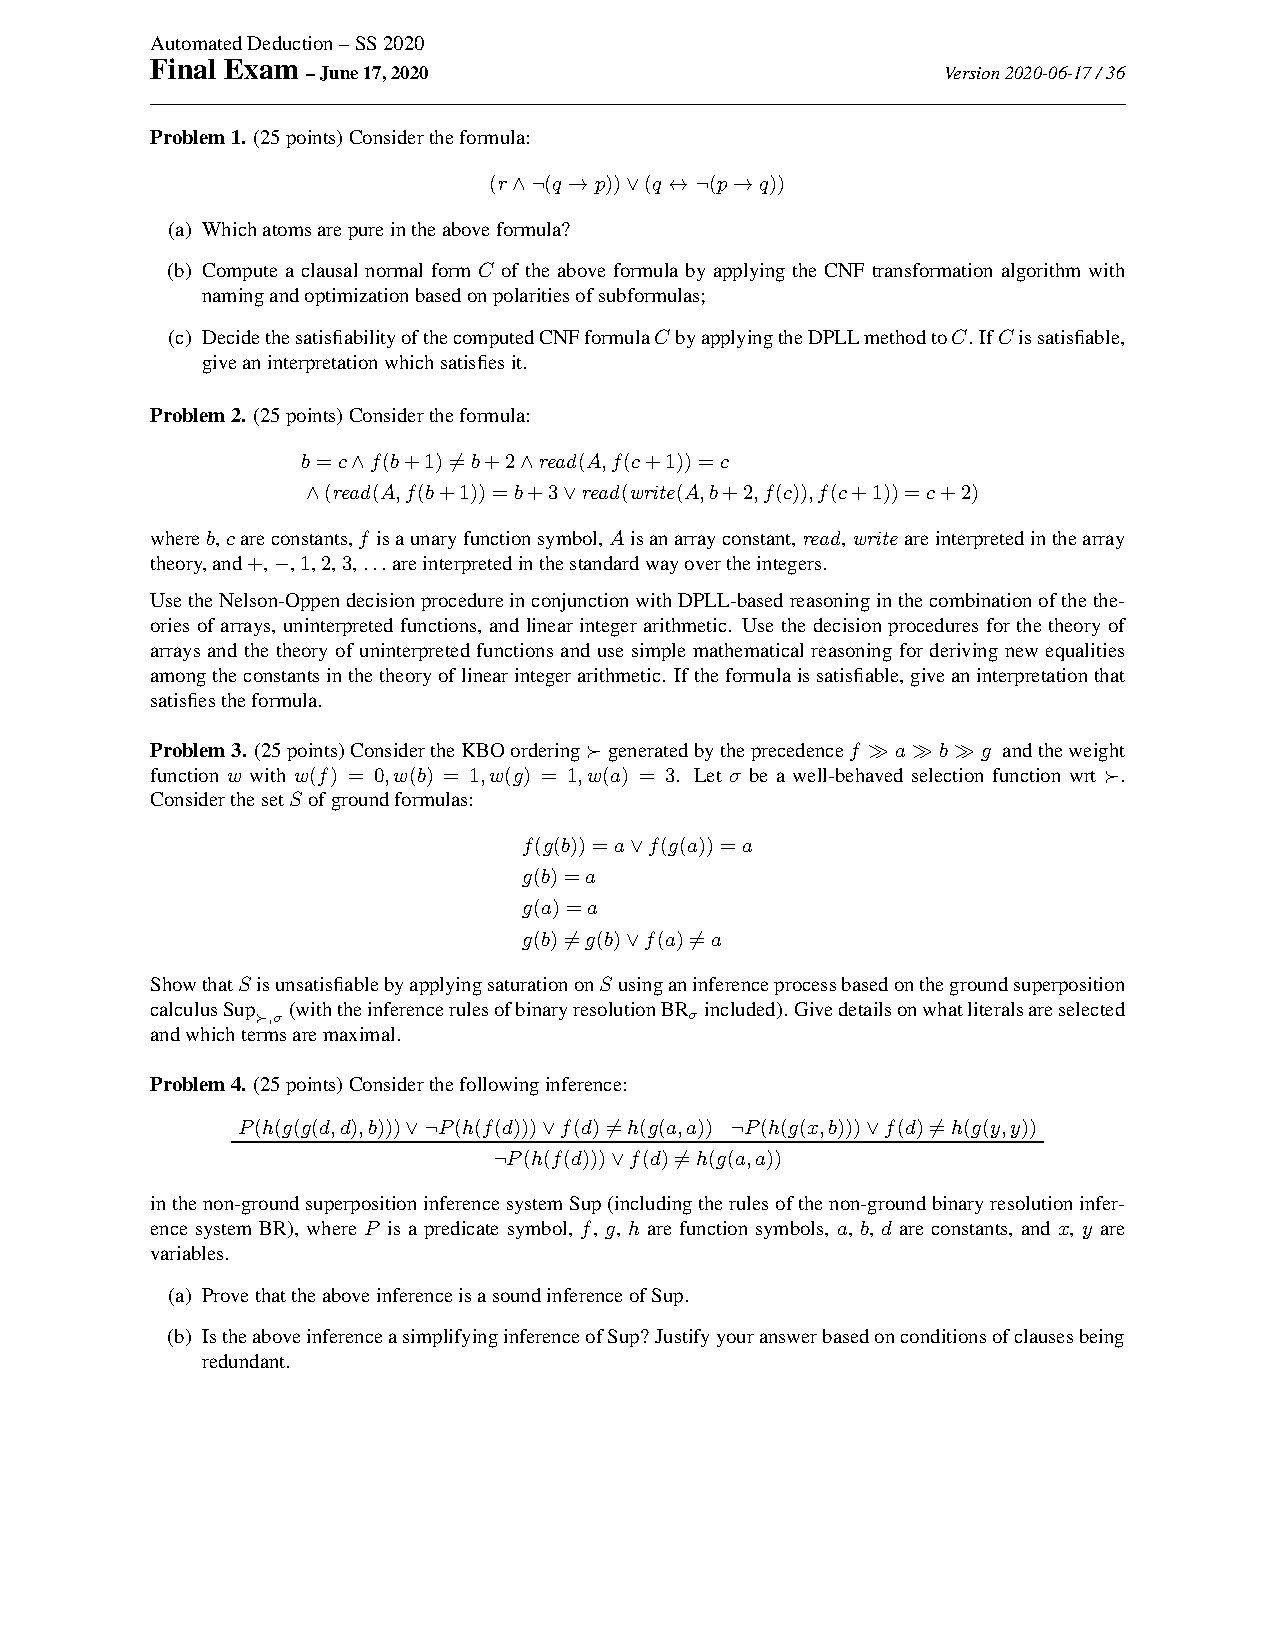
\includegraphics[page=1,width=1.5\textwidth]{./exam-36.pdf}
%}
\newpage
\clearpage

\section{Appendix B}\label{appendixB}
\subsection{Random Problem Generation}\label{appB:SAT}

As we alluded to in Section~\ref{sec:sat},
some issues may arise if the restrictions on the randomly generated formula are too strict:
\begin{itemize}
    \item
        The sample space might be empty or very sparse.
        In practice, this manifests as the generator seemingly getting stuck,
        usually resulting in the process being killed by the user. 
        For example,
        consider the restriction on polarities of propositional
        variables. % (Sect.~\ref{sec:sat}).
        Combined with the other restrictions,
        it is impossible to get a formula that contains atomic proposition
        of purely positive and purely negative polarity at the same time.

    \item
        The second issue manifests less drastically but is perhaps more problematic:
        the sample space may be too uniform,
        leading to the generation of trivial and/or very similar
        formulas. 
        In particular, we encountered this problem
        when we restricted the number of models to exactly one, or zero.
        We note that there simply are not that many ways to rule out 8 interpretations
        using only 7 connectives.
\end{itemize}





Regarding the filtering of generated formulas using the constraints discussed in Section~\ref{sec:satfo},
we did not require very efficient algorithms since
the formulas under consideration are very small.
For example, for the restriction on the number of models we used a naive satisfiability test
based on evaluating the formula under each possible interpretation.
An advantage of this is that the addition of new filters/constraints is relatively easy.




For the random problem generation setting of Section~\ref{sec:satfo},
we used design principles from the Haskell library
QuickCheck~\cite{ClaessenHughes:2000:QuickCheck}.
%which we used for the first prototype.
However, because of our many filtering criteria, we wanted the generator to support backtracking.
To this end,
we created a simple mtl-style typeclass \texttt{MonadChoose}
with a single primitive operation \texttt{choose} for choosing an element from a list of possible choices:
\lstset{
    language=Haskell,
    basicstyle=\small\ttfamily,
    deletekeywords={MonadPlus,filter,length},
    columns=fixed,
}
\begin{lstlisting}
class MonadPlus m => MonadChoose m where
  -- Choose element with uniform probability
  choose :: [a] -> m a
\end{lstlisting}

Our generator implementations are generic over the monad, constrained by \texttt{MonadChoose}.
The following listing shows (a slightly simplified) part of the inference generator
discussed in Section~\ref{sec:fo}.
\begin{lstlisting}
genExamInference :: MonadChoose m => m Inference
genExamInference = do
  -- Define signature (partially omitted)
  let vars = ["x", "y", "z"]
  let opts = GenOptions{ vars = vars, ... }

  -- Choose variables to appear in l1 and l2
  v1 <- choose vars
  v2 <- choose (filter (/= v1) vars)

  -- Generate literals
  -- l1: exactly one occurrence of v1
  l1 <- mfilter ((==1) . length . toListOf variables)
        $ genUninterpretedLiteral opts{ vars = [v1] }
  -- l2: at least two occurrences of v2
  l2 <- mfilter ((>=2) . length . toListOf variables)
        $ genEqualityLiteral opts{ vars = [v2] }
  -- l3: ground literal
  l3 <- genUninterpretedLiteral opts{ vars = [] }

  -- [rest omitted]
  return inference
\end{lstlisting}



We used two concrete implementations to evaluate generators:
\begin{enumerate}
    \item
        \texttt{RandomChoice}, a monad that implements \texttt{choose}
        as uniform random choice with backtracking support.
        Conceptually, this is like the standard list monad
        where \texttt{choose} works like the regular monadic bind for lists
        except that it shuffles the list with a random permutation first.
        This evaluation method is used to generate random exams.
    \item
        The standard list monad to enumerate the sample space.
        This second evaluation method helps verifying that the sample space is sufficiently large.
\end{enumerate}

\subsection{Weights and Precedences for Ground Superposition}\label{appB:FO}

The weights and precedences used to generate the KBOs for the superposition problem
from Section~\ref{sec:gs}
are displayed in Table~\ref{tab:ground-sup}.
The upper part of the table shows all weight and precedence combinations,
denoted as $w_{i, I}, p_{i, I}$ for $i \in \{1, 2, 3, 4\}$
and $I \in \{f, g\}$ (for convenience, the table contains both $w_{i, f}$
and $w_{i, g}$, as well as $p_{i, f}$ and $p_{i, g}$ for all values of~$i$).
The lower part of the table displays the values of $i_1, I_1; i_2, I_2$; and $i_3, I_3$,
corresponding to the three weight and precedence combinations selected for
each instance of the clause set.

\begin{table}
\begin{center}
\begin{tabular}{r@{\hskip 0.5em}c c c c@{\hskip 0.5em} |@{\hskip 0.5em} l@{\hskip 1em} ||@{\hskip 0.5em} r@{\hskip 0.5em} c c c c@{\hskip 0.5em} |@{\hskip 0.5em} l}
  weight of: & $f$ & $g$ & $a$ & $b$ & precedence
  & weight of: & $f$ & $g$ & $a$ & $b$ & precedence \\ \hline
  $w_{1,f}:$  & 1   & 3   & 2   & 1   & $p_{1,f}: a \gg b \gg f \gg g$ &
  $w_{1,g}:$  & 3   & 1   & 2   & 1   & $p_{1,g}: a \gg b \gg g \gg f$ \\ \hline
  $w_{2,f}:$  & 0   & 3   & 2   & 1   & $p_{2,f}: f \gg a \gg g \gg b$ &
  $w_{2,g}:$  & 3   & 0   & 2   & 1   & $p_{2,g}: g \gg a \gg f \gg b$ \\ \hline
  $w_{3,f}:$  & 0   & 1   & 3   & 1   & $p_{3,f}: f \gg a \gg b \gg g$ &
  $w_{3,g}:$  & 1   & 0   & 3   & 1   & $p_{3,g}: g \gg a \gg b \gg f$ \\ \hline
  $w_{4,f}:$  & 1   & 2   & 3   & 1   & $p_{4,f}: g \gg f \gg a \gg b$ &
  $w_{4,g}:$  & 2   & 1   & 3   & 1   & $p_{4,g}: f \gg g \gg a \gg b$ \\ \hline
  % original table:
  %$w_1(h_1) = w_1(b) = 1, w_1(a) = 2, w_1(h_2) = 3$ & \quad $p_1: a \gg b \gg h_1 \gg h_2$ \\
  %$w_2(h_1) = 0, w_2(b) = 1, w_2(a) = 2, w_2(h_2) = 3$ & \quad $p_2: h_1 \gg a \gg h_2 \gg b$ \\
  %$w_3(h_1) = 0, w_3(b) = w_3(h_2) = 1, w_3(a) = 3$ & \quad $p_3: h_1 \gg a \gg b \gg h_2$ \\
  %$w_4(b) = w_4(h_1) = 1, w_4(h_2) = 2, w_4(a) = 3$ & \quad $p_4: h_2 \gg h_1 \gg a \gg b$ \\
\end{tabular}

\hspace*{0.5em}

\begin{tabular}{l@{\hskip 1.05em} || c | c | c}
\hline
condition & $i_1, I_1$ & $i_2, I_2$ & $i_3, I_3$ \\ \hline
$F \not = G$ and $X \not= Y$ & $1,E$ & $2, E$ & $3, E$ \\
$F \not = G$ and $X = Y$ & $1, H$ & $2, E$ & $4, H$ \\
$F = G$ and $X \not= Y$ & $1, H$ & $2, H$ & $3, E$
\end{tabular}
\hspace*{0.5em}
\caption{Weights and precedences for the ground superposition problem.}
\label{tab:ground-sup}
\end{center}
\end{table}



\end{document}
